\documentclass{article}

% Language setting
% Replace `english' with e.g. `spanish' to change the document language
\usepackage[english]{babel}

% Set page size and margins
% Replace `letterpaper' with `a4paper' for UK/EU standard size
\usepackage[letterpaper,top=2cm,bottom=2cm,left=3cm,right=3cm,marginparwidth=1.75cm]{geometry}

% Useful packages
\usepackage{amsmath}
\usepackage{graphicx}
\usepackage{subcaption} % For subfigures
\usepackage[colorlinks=true, allcolors=blue]{hyperref}
\usepackage{float}

\title{Machine Learning Exercise 1}
\author{Amélie Assmayr (12007770) \and
        Konstantinos Damanakis (12106343) \and
        Teresa Schuch (12007762)}

\begin{document}
\maketitle

\section{Introduction}
This report outlines the experimental design of the application of different classification algorithms across four diverse datasets. The goals is to show the trends in classifier performance, based on dataset properties like size and dimensionality, as well as the impact of preprocessing steps like scaling and different parameter settings.

The report is structured as followed: In Section 2 we introduce the chosen classifier and shortly explain their functionality. Section 3 describes the performance metrics used to evaluate each model across different configurations. Section 4 details the main characteristics of each datasets, the preprocessing steps applied and presents the evaluation results. Finally, in Section 5 discusses the main findings and insights drawn from the analysis.

\section{Classifiers}
We selected three distinct classifiers: an ensemble method (Random Forest), a margin-based method (SVM), and a distance-based method (KNN).

\subsection{K-nearest-neighbors}
\subsection{Random Forest}
Random Forest (RF) is an ensemble  method based on decision trees. It builds multiple decision trees during training and combines their prediction for more accurate and stable results. We chose this algorithm because it is good at handling both numerical and categorical data, making it a robust choice for diverse datasets. Furthermore due to its functionality Random Forests are resistant to overfitting, requires minimal preprocessing and offers offers flexibility through parameter tuning. This makes it useful also for complex and large datasets.


\subsection{Support Vector Machines}

\section{Performance Measures}
In order to ensure that the performance of the classifiers can be meaningfully compared, the following steps were taken:
\begin{itemize}
    \item \textbf{Dataset:} The same train/test splits were used across all classifiers to ensure consistency across all experiments.
    \item \textbf{Parameter changes:} To compare how one hyperparameter affects the outcome, only a single hyperparameter was changed at a time.
    \item \textbf{Baseline comparison:} The classifiers can be compared based on their baseline performance where no hyperparameters are set.
\end{itemize}

\subsection{Training time}
raining time is important because larger or more complex models often give better results. However, it's important to check if the improvement is worth the additional training time.

\subsection{Accuracy}
$\text{Formula} = \frac{TP + TN}{TP + TN + FP + FN}$

Accuracy measures the proportion of correctly classified instances out of all instances. While it’s easy to interpret, it can be misleading, especially in imbalanced datasets, because it doesn't distinguish between false positives and false negatives.

\subsection{Precision}
$\text{Formula} = \frac{TP}{TP + FP}$

Precision measures how many of the positive predictions were actually correct and therefore measures the model’s ability to precisely identify relevant instances within the data. Either by class or averaged across all classes.

\subsection{Recall}
$\text{Formula} = \frac{TP}{TP + FN}$

Recall measures how many true positive cases the model was able to identify. Either by class or averaged
across all classes.

\subsection{F1-score}

$\text{Formula}  = 2 \times \frac{\text{Precision} \times \text{Recall}}{\text{Precision} + \text{Recall}}$

The F1-score balances precision and recall. It thereby gives accurate results even if the dataset is skewed towards certain target classes. It might however be more difficult to immediately understand the score.

\section{Datasets}
PLOTS: Correlation and Barplot of Target

\subsection{Congressional Voting}
This dataset contains the voting records of U.S. House of Representatives members. It has 18 columns and 218 observation, making it one of the smaller datasets used. It includes voting data on 16 key issues, where each vote is recorded as "Yes," "No," or "Unknown." The target variable indicates whether each representative is a Democrat or Republican. Additionally, there is an ID column for each representative. Below, the distribution of the target variable and of the vote counts for each issue can be seen. It shows that the target variable is nearly 50:50 balanced. Furthermore it reveals that the dataset contains missing values (="Unknown") in each of the voting column which have to be handled in the preprocessing.

\begin{figure}[H]
    \centering
    \begin{subfigure}[b]{0.45\textwidth}
        \centering
        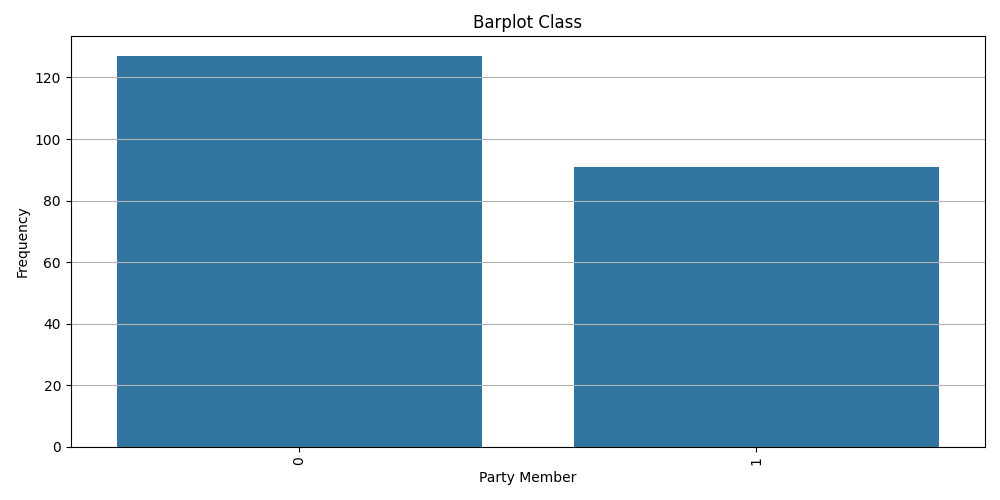
\includegraphics[width=\linewidth, height=5cm]{barplot_target.png} 
        \caption{Barplot of target}
        \label{fig:figure1}
    \end{subfigure}
    \hspace{0.05\textwidth} % Adjust space between figures
    \begin{subfigure}[b]{0.45\textwidth}
        \centering
        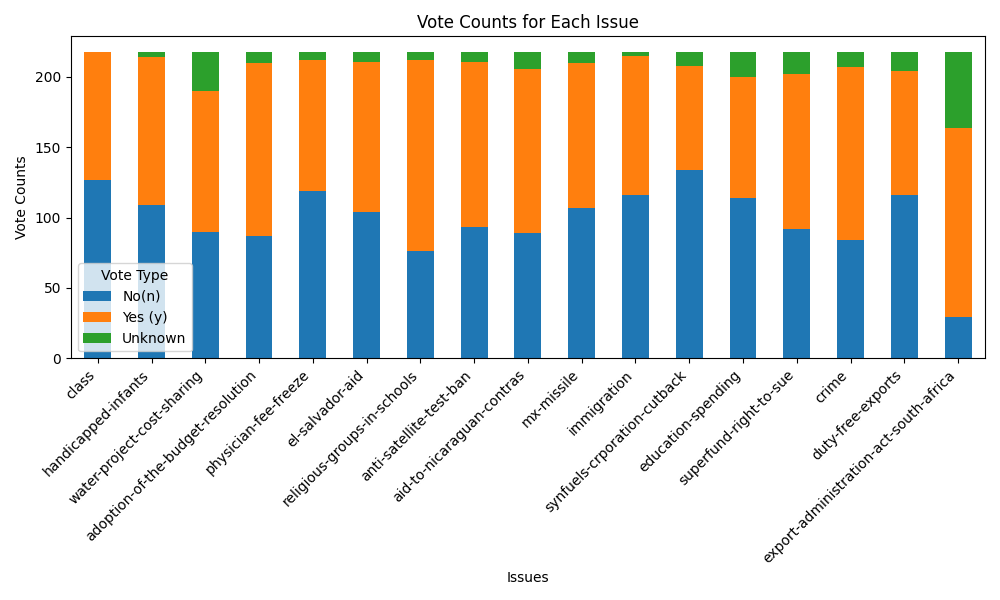
\includegraphics[width=\linewidth]{stacked_barplot.png} 
        \caption{stacked Barplot votes}
        \label{fig:figure2}
    \end{subfigure}
    \label{fig:two_figures}
\end{figure}


\subsubsection{Preprocessing}
First, a LabelEncoder is applied to convert the categorical variables into a binary format.  For the target variable, Democrats are encoded as 0 and Republicans as 1.  n the vote columns, 'no' is encoded as 0 and 'yes' as 1. Any 'unknown' values are replaced with NaN to mark them as missing. Next, rows with more than half of their values missing are removed from the dataset. The remaining missing values are then imputed by filling them with the most frequent value in each column. Since the dataset consists only of binary data, there is no need for additional transformations like scaling or outlier handling. 

\subsubsection{Results}

The baseline Random Forest classifier has already very high performance across all metrics with scores consistently above 0.95. The 10-fold cross-validation gave slightly better scores, indicating a stable and reliable model across different splits. Therefore adjusting parameters yields only small changes in the results. The highest improvement gave setting the parameter n\_estimators to 200, however this comes with the trade-off of increased training time.

\begin{table}[ht]
\centering
\begin{tabular}{l|c|c|c|c|c|c}
\textbf{Model Parameters} & \textbf{Training Time (s)} & \textbf{Accuracy} & \textbf{Precision} & \textbf{Recall} & \textbf{F1} \\\hline
default (Holdout) & 0.13  & 0.9545 & 0.9545 & 0.9545 & 0.9545 \\
default (Cross-validated) & /  & 0.9675 & 0.9696 & 0.9675 & 0.9675 \\
n\_estimators=200 & 0.2762  & 0.9723 & 0.9739 & 0.9723 & 0.9722 \\
max\_depth=10 & 0.1782  & 0.9675 & 0.9696 & 0.9675 & 0.9675 \\
min\_samples\_leaf=10 & 0.1269  & 0.9537 & 0.9564 & 0.9537 & 0.9537 \\
min\_samples\_split=10 & 0.1269  & 0.9630 & 0.9655 & 0.9630 & 0.9630 \\
\end{tabular}
\caption{Random Forest - Congressional Voting}
\label{tab:Random Forest - Congressional Voting}
\end{table}

\subsection{Amazon Reviews}
\subsubsection{Preprocessing}
\subsubsection{Results}

The baseline random forest classifier achieves moderate performance, with an accuracy of 0.63. Also for this dataset increasing the number of n\_estimators brings the best improvement in terms of accuracy but comes at the cost of longer training times.


\begin{table}[ht]
\centering
\begin{tabular}{l|c|c|c|c|c|c}
\textbf{Model Parameters} & \textbf{Training Time (s)} & \textbf{Accuracy} & \textbf{Precision} & \textbf{Recall} & \textbf{F1} \\\hline
default (Holdout) & 1.5087  & 0.6267 & 0.6633 & 0.6267 & 0.6014 \\
default (Cross-validated) & /  & 0.5947 & 0.5523 & 0.5947 & 0.5448 \\
n\_estimators=200 & 3.1516  & 0.6547 & 0.6280 & 0.6547 & 0.6116 \\
max\_depth=10 & 0.7156  & 0.5373 & 0.4805 & 0.5373 & 0.4758 \\
min\_samples\_leaf=10 & 0.5826  & 0.5107 & 0.4493 & 0.5107 & 0.4438 \\
min\_samples\_split=10 & 1.1777  & 0.6280 & 0.5936 & 0.6280 & 0.5788 \\
\end{tabular}
\caption{Random Forest - Amazon Reviews}
\label{tab:Random Forest - Amazon Reviews}
\end{table}




\subsection{Road Traffic Accidents}
\subsubsection{Preprocessing}
\subsubsection{Results}

For the Road Traffic Accidents dataset, the default random forest classifier performs well, achieving an accuracy of 0.8460. Parameter modification yielded little to no improvement.

\begin{table}[ht]
\centering
\begin{tabular}{l|c|c|c|c|c|c}
\textbf{Model Parameters} & \textbf{Training Time (s)} & \textbf{Accuracy} & \textbf{Precision} & \textbf{Recall} & \textbf{F1} \\\hline
default (Holdout) & 0.8502  & 0.8460 & 0.8078 & 0.8460 & 0.7803 \\
default (Cross-validated) & /  & 0.8498 & 0.8302 & 0.8498 & 0.7865 \\
n\_estimators=200 & 1.8891  & 0.8496 & 0.8295 & 0.8496  & 0.7858 \\
max\_depth=10 & 0.5707  & 0.8480 & 0.8499 & 0.8480 & 0.7803 \\
min\_samples\_leaf=10 & 0.6435  & 0.8467  & 0.7592 & 0.8467 & 0.7768 \\
min\_samples\_split=10 & 0.8960  & 0.8492 & 0.8386 & 0.8492 & 0.7836 \\
\end{tabular}
\caption{Random Forest - Road Traffic Accidents}
\label{tab:Random Forest - Road Traffic Accidents}
\end{table}

\subsubsection{Impact of Balancing}
The data exhibits significant class imbalance. This can lead to misclassifying the minority class.To mitigate this issue, the Synthetic Minority Over-sampling Technique (SMOTE) is applied to balance the representation of the minority class in the data.

The following plots show how balancing affect the accuracy of the three classifiers. The Random Forest plot demonstrates that balancing has a positive effect with the accuracy of the balanced dataset is consistently higher.

\begin{figure}[H]
\centering
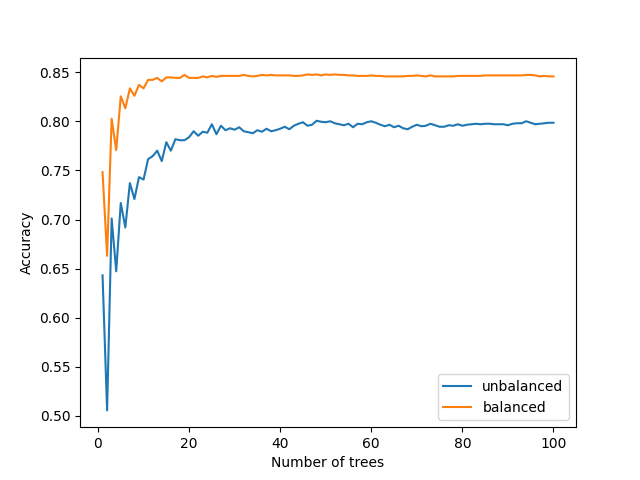
\includegraphics[width=0.5\linewidth]{RTA_balancing.png}
\caption{\label{fig:hist:price}Impact of balancing on Random Forest}
\end{figure}


\subsection{Machine Failure}
\subsubsection{Preprocessing}
\subsubsection{Results}

The default Random Forest Classifier for the Machine Failure dataset achieved an accuracy of 0.8940. Interesting here is that
adjusting the min\_samples\_leaf parameter to 10, resulted in the highest improvement. This increased the accuracy to 0.9127 with only a slightly higher training time.

\begin{table}[ht]
\centering
\begin{tabular}{l|c|c|c|c|c|c}
\textbf{Model Parameters} & \textbf{Training Time (s)} & \textbf{Accuracy} & \textbf{Precision} & \textbf{Recall} & \textbf{F1} \\\hline
default (Holdout) & 0.1592  & 0.8940 & 0.8940 & 0.8940 & 0.8939 \\
default (Cross-validated) & /  & 0.9034 & 0.9056 & 0.9034 & 0.9032 \\
n\_estimators=200 & 0.3556  & 0.9034 & 0.9054 & 0.9034  & 0.9033 \\
max\_depth=10 & 0.5707  & 0.8480 & 0.8499 & 0.8480 & 0.7803 \\
min\_samples\_leaf=10 & 0.1689  & 0.9127  & 0.9156 & 0.9127  & 0.9129 \\
min\_samples\_split=10 & 0.1568  & 0.9061 & 0.9079 & 0.9061 & 0.9061 \\
\end{tabular}
\caption{Random Forest - Machine Failure}
\label{tab:Random Forest - Machine Failure}
\end{table}

\subsubsection{Impact of Scaling}

To investigate how the classifiers are affected by scaling we apply the Standardscaler to the machine failure data. This standardize the features by removing the mean and scaling to unit variance.

It reveals that Random Forest is not affected by scaling.

\begin{figure}[H]
\centering
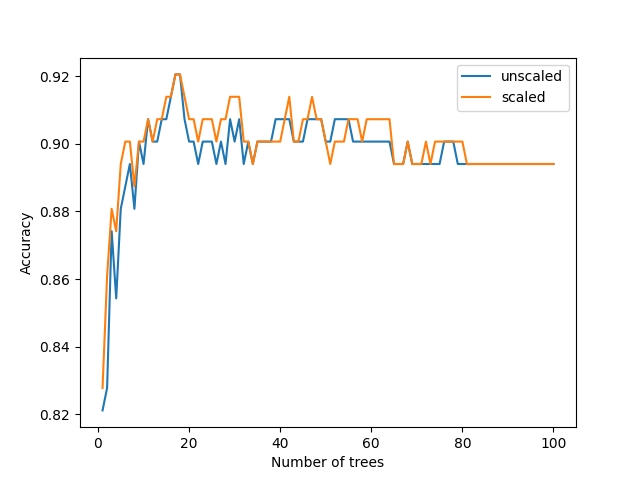
\includegraphics[width=0.5\linewidth]{Machine_scaling.png}
\caption{\label{fig:hist:price}Impact of scaling on Random Forest}
\end{figure}



\section{Discussion of Findings}




\section{Notes}

\end{document}